\documentclass{article}
\usepackage{tikz}
\usetikzlibrary{positioning}
\begin{document}
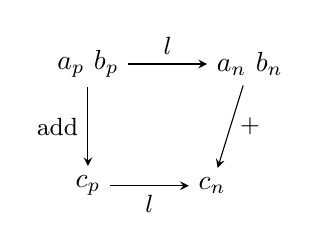
\begin{tikzpicture}
  % Tell it where the nodes are
  \node (A) {$a_p$ $b_p$};
  \node (B) [below=of A] {$c_p$};
  \node (C) [right=of A] {$a_n$ $b_n$};
  \node (D) [right=of B] {      $c_n$};
  % Tell it what arrows to draw
  \draw[-stealth] (A)-- node[left] {\small $\mbox{add}$} (B);
  \draw[-stealth] (B)-- node [below] {\small $l$} (D);
  \draw[-stealth] (A)-- node [above] {\small $l$} (C);
  \draw[-stealth] (C)-- node [right] {\small $+$} (D);
\end{tikzpicture}
\end{document}
